\section{Fall 3: Hund}
\label{sec:testcase-dog}
Im dritten Testfall wird versucht mit neuen Bildern einen Hund in einem Körbchen zu rekonstruieren, der in \cref{fig:dog-image} zu sehen ist.

Die \cref{tab:dog-results} zeigt die Ergebnisse der Rekonstruktion.
In allen Bildpaaren ist der Matches höher als im ersten Testfall.
Betracht man jedoch in \cref{fig:dog-first-pair-with-matches} wo die Matches liegen, dann fällt auf, dass keine auf dem Hund liegen.
Stattdessen befinden sich alle Matches auf dem Teppich.
Das Modell in Blender zeigt dem entsprechend nur eine Fläche, die aus beige Punkten besteht.
Das Problem in diesem Testfall ist wie beim Auto und dem Sitzkissen des Sessels, dass der Hund keine auffälligen Kanten besitzt, die als Feature erkannt werden.
Des Weiteren ist das Aufnehmen der Fotos in diesem Fall problematisch. 
Im Vergleich zum Sessel oder dem Auto ist es schwierig mehrere und gute Bilder von dem Hund zu machen, ohne dass er sich bewegt. 
Es war nicht möglich den Hund stehend zu fotografieren, da er entweder weiter gelaufen ist oder den Kopf mit der Kamera bewegt hat.
Die Fotos konnten erst dann gemacht werden, wenn der Hund zufällig im Körbchen gelegen hat und sich nicht beweg hat.

\begin{figure}
    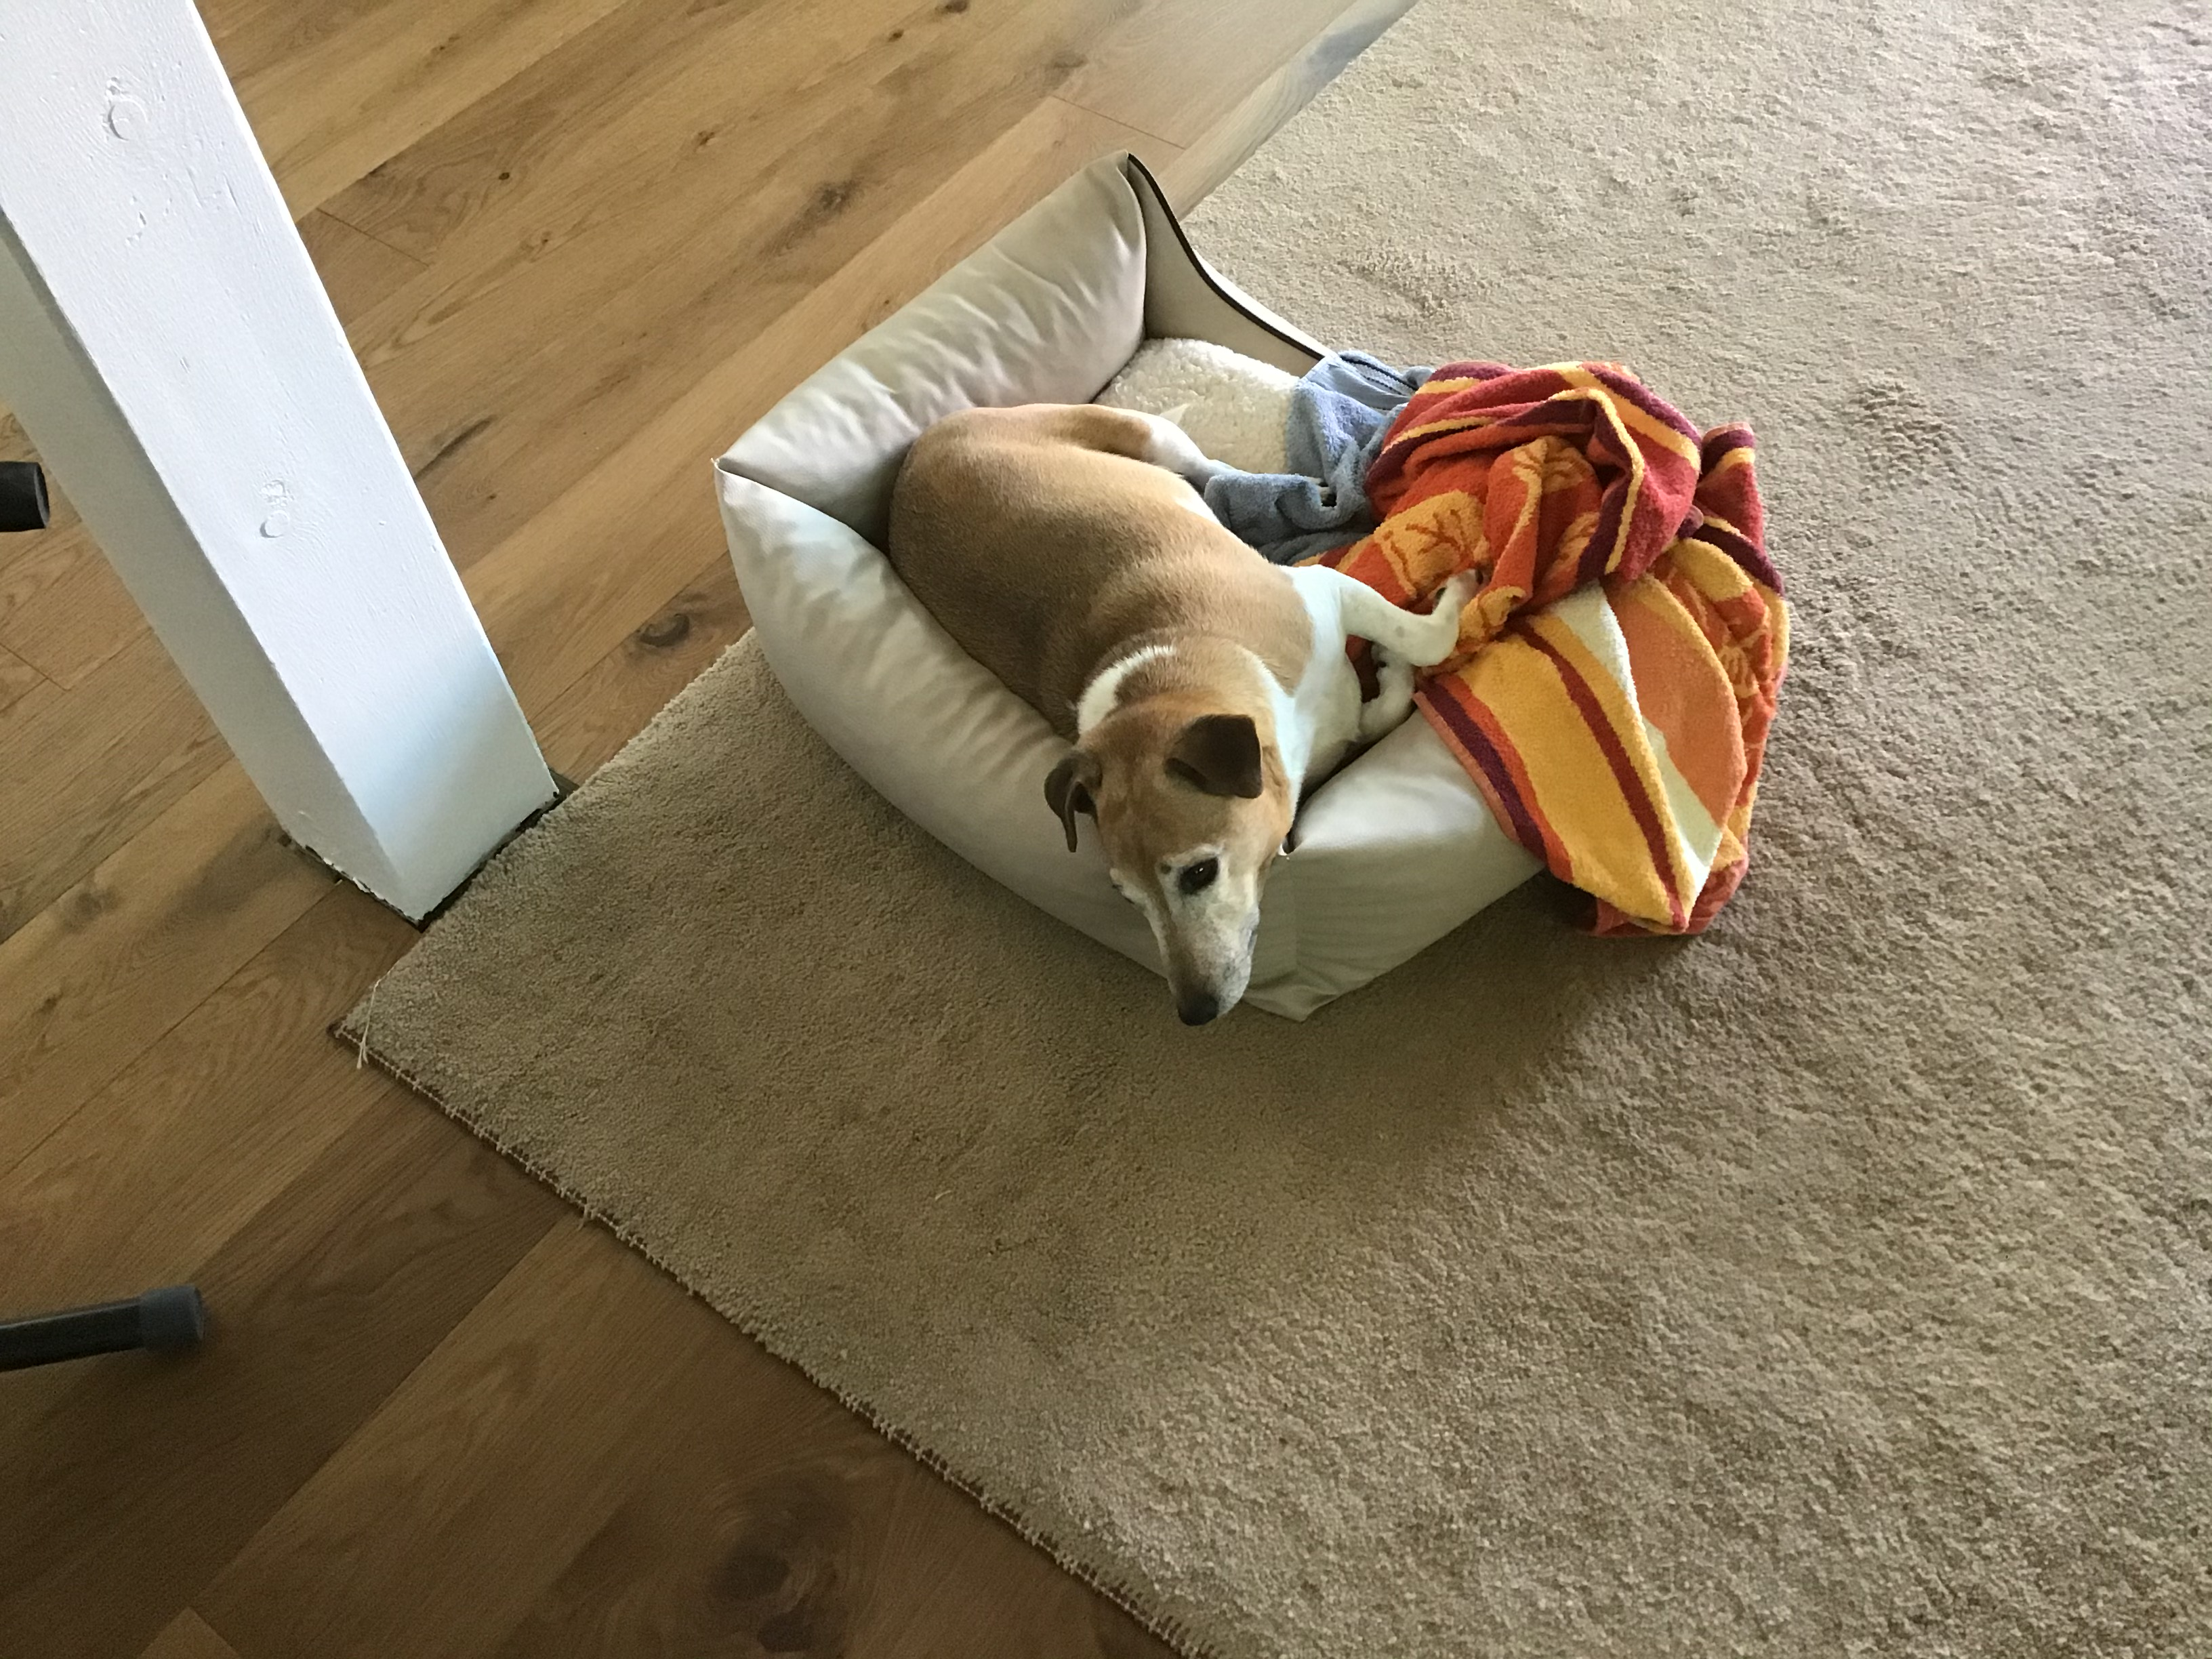
\includegraphics[width=\textwidth]{src/img/dog.jpg}
    \caption{Der Hund, genannt Sam, der im Körbchen liegt und rekonstruiert wird.}
    \label{fig:dog-image}
\end{figure}

\begin{table}
    \begin{tabularx}{\textwidth}{cXXXX}
        \toprule
        Bildpaar &  Anzahl der Matches & Anzahl der Weltpunkte & Anzahl der Weltpunkte für Skalierung & angewandte Skalierung \\ 
        \midrule
        1 & 4.799 & 4.786 & -  & - \\
        2 & 6.450 & 6.421 & 2.127 & 0,835131 \\
        3 & 6.525 & 6.472 & 2.763 & 0,892978 \\
        4 & 7.520 & 7.489 & 2.867 & 0,975344 \\
        5 & 7.462 & 7.444 & 3.215 & 0,801014 \\
        6 & 3.024 & 2.984 & 1.651 & 0,93856  \\
        7 & 6.071 & 6.009 & 1.337 & 1,42251  \\
        8 & 7.893 & 7.874 & 3.091 & 0,707064 \\
        9 & 6.917 & 4.350 & 1.924 & 1,01307  \\
        \midrule
        Summe & 56.661 & 53.829 & 18.975 & - \\
        \bottomrule
    \end{tabularx}
    \caption{Ergebnis der Rekonstruktion der neun Hundebilder}
    \label{tab:dog-results}
\end{table}

\begin{figure}
    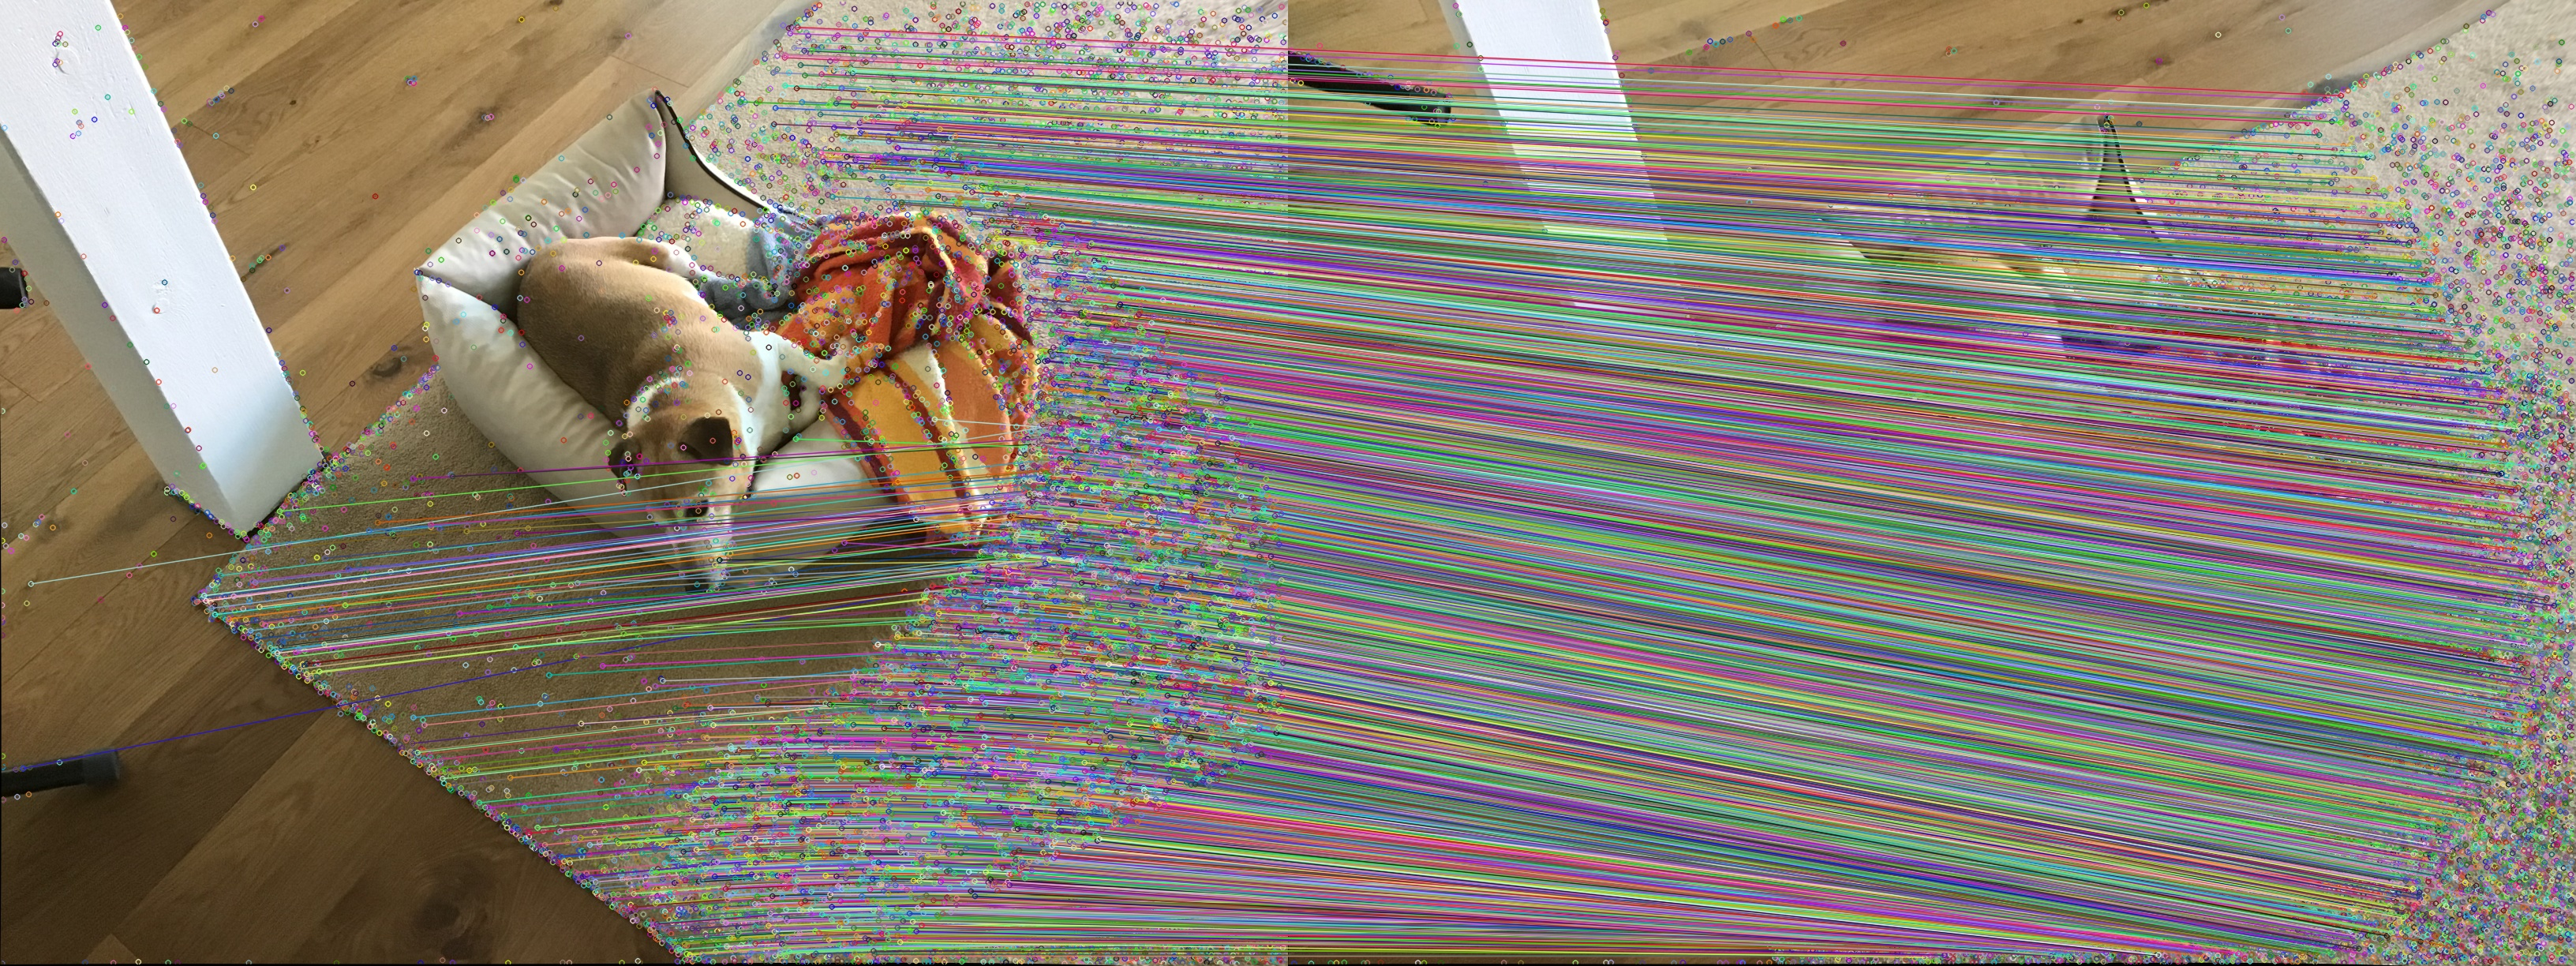
\includegraphics[width=\textwidth]{src/img/dog_first_pair_with_matches.jpg}
    \caption{Das erste der neun 8 Bildpaare, das die Keypoints und ihre Matches zeigt.}
    \label{fig:dog-first-pair-with-matches}
\end{figure}

\begin{figure}
    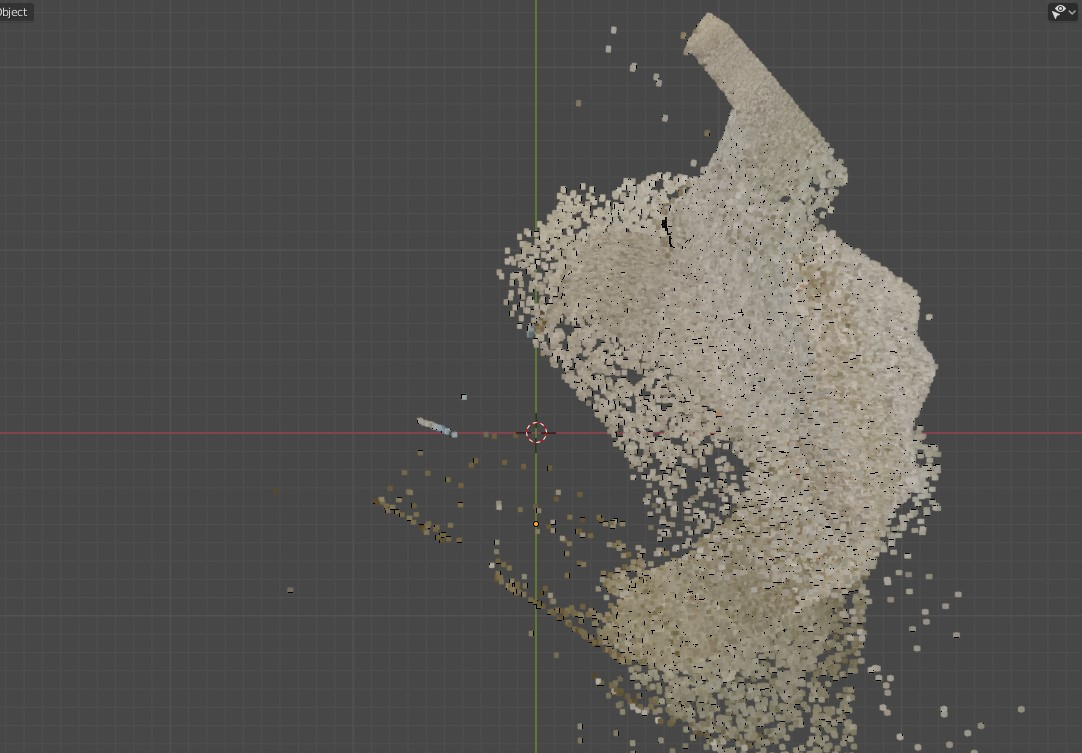
\includegraphics[width=\textwidth]{src/img/dog_model.jpg}
    \caption{Die rekonstruierten Punkte aus den Hundebildern. Das Bild zeigt das Modell ungefähr aus der Position der ersten Kamera.}
    \label{fig:dog-model}
\end{figure}

\begin{figure}
    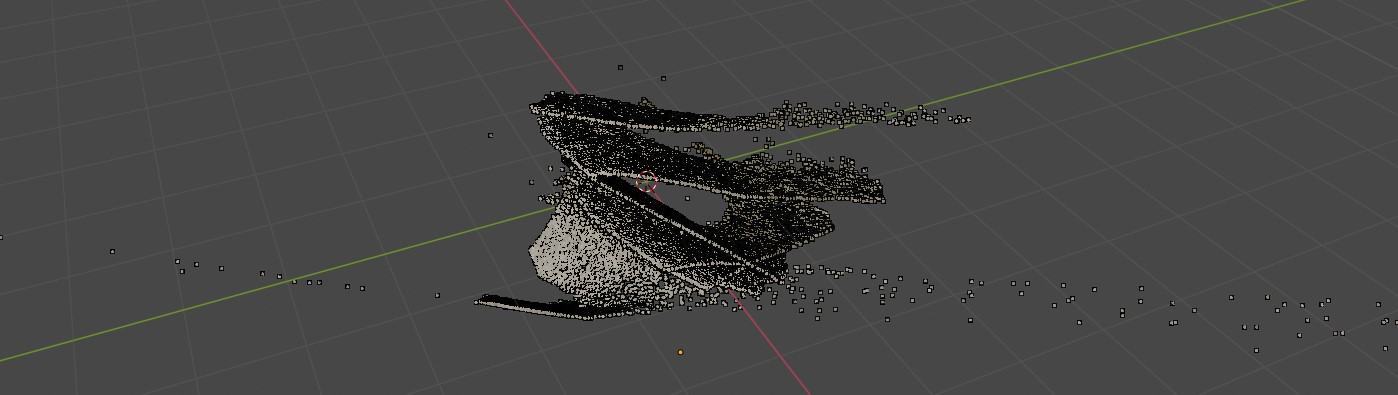
\includegraphics[width=\textwidth]{src/img/dog_model_2.jpg}
    \caption{Die rekonstruierten Punkte aus den Hundebildern. Das Bild zeigt das Modell von der Seite.}
    \label{fig:dog-model-2}
\end{figure}
